\documentclass{svproc}

% Packages
\usepackage{cite}
\usepackage{amsmath,amssymb,amsfonts}
\usepackage{algorithmic}
\usepackage{graphicx}
\usepackage{textcomp}
\usepackage{xcolor}
\usepackage{booktabs}
\usepackage{multirow}
\usepackage{array}
\usepackage[hidelinks]{hyperref}
\usepackage{tabularx}

% Space tightening for floats
\setlength{\textfloatsep}{8pt plus 2pt minus 2pt}
\setlength{\intextsep}{6pt plus 2pt minus 2pt}
\setlength{\floatsep}{6pt plus 2pt minus 2pt}
\setlength{\parskip}{0pt}

% Custom commands
\newcommand{\modelname}{FC-MT-LSTM}
\newcommand{\eg}{\textit{e.g.}}
\newcommand{\ie}{\textit{i.e.}}
\newcommand{\etal}{\textit{et al.}}
\def\BibTeX{{\rm B\kern-.05em{\sc i\kern-.025em b}\kern-.08em
T\kern-.1667em\lower.7ex\hbox{E}\kern-.125emX}}

\begin{document}

\title{Fairness-Constrained Multi-Task Learning for Crime Prediction:\\
Addressing Bias Against Vulnerable Populations in Criminal Justice Systems}

\author{Rishabh Singh \{rs2198908@gmail.com\}$^{1}$ \and
Nehul Agarwal \{nehulagarwal15@gmail.com\}$^{1}$ \and
Farah Masoodi \{farahmasodi613@gmail.com\}$^{1}$ \and
Archit Raghav \{architraghav2004@gmail.com\}$^{1}$ \and
Geetanjali Tyagi \{geetanjt@srmist.edu.in\}$^{1}$}

\institute{
$^1$ Department of Computer Science and Engineering\\
SRM Institute of Science and Technology\\
Delhi NCR Campus, Modinagar, Uttar Pradesh, India\\[1ex]
}

\titlerunning{FC-MT-LSTM}
\authorrunning{ }
\maketitle

% ------------------------------------------------------------------
\section{Abstract}
% ------------------------------------------------------------------

\noindent\textbf{Background:} Crime forecasting is becoming a key element in how law-enforcement agencies allocate limited resources, yet many predictive systems unintentionally replicate long-standing structural biases against vulnerable communities.

\noindent\textbf{Objective:} This paper presents a Fairness-Constrained Multi-Task Long Short-Term Memory (\modelname{}) framework that seeks to maintain high predictive accuracy while improving equity of performance across protected demographic groups.

\noindent\textbf{Materials and Methods:} We use National Crime Records Bureau (NCRB) data for India from 2017--2022, covering 36 states and union territories, over 700 districts, and 21{,}067 records for Scheduled Castes (SC), Scheduled Tribes (ST), women, and children. Built six baseline models for comparison against our \modelname{}; which are SARIMA, Prophet, Random Forest, XGBoost, CNN-LSTM, and a Transformer. Fairness-regularised loss trained the itegrated architecture of spatial convolutional layers, an attention-based bidirectional LSTM, a shared encoder, and group-specific decoder

\noindent\textbf{Results:} Retention of fairness accuracy (MAE: 6.54, R$^2$: 0.9922) with balanced errors among protected goups (Fairness Ratio:1.99) is achieved by \modelname{}. As for baseline models in groupwise error display huge differences, upto 3.7--4.7$\times$.

\noindent\textbf{Conclusion:} For bieng fair in crime forecasting a framework is proposed which is implemented in both PyTorch and TensorFlow.

\keywords{Algorithmic fairness, crime prediction, multi-task learning, LSTM, deep learning, protected groups, bias mitigation}

% ------------------------------------------------------------------
\section{Introduction}
% ------------------------------------------------------------------

Criminal justice is adopting the use of algorithmic instruments to make decisions related to patrol planning, resource allocation, and crime prevention \cite{perry2013predictive}. Machine learning algorithms which have been trained on past information of crimes, socioeconomic trends and time trends, can predict future crime with remarkable accuracy on a macro-level. Nevertheless, the statistics behind these systems also encode some historic inequities in policing, reporting behaviour, and social conditions at large [2,3]. When predictive systems are engaged without express conditions on fairness, they may reinforce disparities that already exist by directing attention and enforcement to those communities already under heavy surveillance, and under-serve vulnerable populations \cite{lum2016predict,richardson2019dirty}.

Majority of crime prediction systems only optimise standard accuracy indices like Mean Absolute Error (MAE), R-squared or Root Mean Square Error (RMSE). By concentrating on these goals, it is possible to obscure inequality within the group: a model can be biased in its perception of crimes against women and children, or provide significantly different error distributions in different demographic groups but still appear right on a city or country scale. When patrols, investigations or social interventions are assigned based on these forecasts, the miscalibration of different groups will threaten to reinforce historical injustices instead of reducing them.

Table~\ref{tab:literature_survey} outlines some important areas of previous research on crime prediction and algorithmic fairness.
This blueprint seeks to develop a crime predictive system that can be competitive on aggregate accuracy and clearly limits discrepancies within covered groups. Instead of figuring out two entirely different models, which loses common structure in crime processes, we propose a fairness-constrained multi-task architecture that learns a shared representation of crime patterns with group specific distinctions. The model is able to take advantage of shared by the formulation of information and directly punishing regimes where there is a consistent modeling of one group of people who is always punished worse than the rest of the users.

\subsection{Research Objectives}

The research questions of this paper are to investigate and control the trade-off between justice and accuracy in predicting crime:
\begin{enumerate}
\item Develop a deep learning framework that jointly models crime patterns for four protected groups: SC, ST, women, and children.Develop an intensive learning to simultaneously model crime trends among four guarded groups: SC, ST, women, and children.
\item Apply fairness constraints in training to ensure the gap in prediction error among vulnerable groups is sanctioned.
\item Compare the performance of fairness-conscious training and traditional accuracy based evaluation on actual crime data.
\item Compare the proposed \modelname{} model to six powerful baselines in the statistical, ensemble, and deep learning models.
\item Demonstrate how such a model may be used to inform more balanced distribution of policing and prevention resources on practice.
\end{enumerate}

\subsection{Contributions}

The main contributions are:
\begin{itemize}
\item \textbf{Novel Architecture}: \modelname{}, integration of spatial CNNs, attention-guided LSTMs, a shared encoder, and group-specific decoders facilitated with a fairness-aware regularised loss.
\item \textbf{Comprehensive Benchmarking}: Evaluating parallelly against six strong baselines spanning statistical models (SARIMA, Prophet), group based (Random Forest, XGBoost), and deep learning models (CNN-LSTM, Transformer).
\item \textbf{Rigorous Fairness Assessment}: Disparity revealing group specific metrics in prediction performance across SC, ST, women, and children.
\item \textbf{Real-World Data Resource}: Six years of NCRB crime records from India, annotated for protected categories across 700+ districts.
\item \textbf{Deployment-Ready Implementation}: A functional code in both PyTorch and TensorFlow, built for adaptive use in real-world.
\end{itemize}

% ------------------------------------------------------------------
\section{Related Work}
% ------------------------------------------------------------------

\subsection{Crime Prediction Models}

Crime prediction techniques have progressed from basic time-series models to sophisticated spatial-temporal and deep learning frameworks. Initial efforts leaned on ARIMA-style approaches to model temporal patterns in crime counts \cite{box2015time}. Later work incorporated spatial dimensions—for instance, via geographically weighted regression—to account for location-specific effects \cite{anselin2000spatial}. Tree-based techniques like Random Forests and gradient-boosted trees excel at capturing non-linear links between socio-economic factors and crime rates, particularly with tabular data \cite{breiman2001random,chen2016xgboost}. Tools such as Prophet, which manage missing values and pronounced seasonality, have enabled scalable crime forecasting \cite{taylor2018forecasting}. In recent years, CNNs applied to crime heatmaps, LSTMs for extended temporal dependencies, and Transformer architectures leveraging self-attention have delivered top-tier accuracy \cite{huang2018deepcrime,hochreiter1997long,vaswani2017attention}. Still, these methods tend to focus narrowly on minimising overall error, rarely assessing whether their performance holds up fairly across different demographic groups.

\subsection{Algorithmic Fairness in Criminal Justice}

Algorithmic tools in criminal justice have raised serious concerns after evidence of racial and demographic bias in risk assessments such as COMPAS \cite{angwin2016machine}. This has led to a wave of work that formalises different fairness notions, explores inherent trade-offs, and proposes technical interventions \cite{dressel2018accuracy,verma2018fairness,kleinberg2016inherent}. Methods span pre-processing (modifying data distributions), in-processing (adding fairness constraints during training), and post-processing (adjusting outputs to satisfy fairness criteria) \cite{kamiran2012data,zafar2017fairness,hardt2016equality}. Recent studies on crime forecasting consider reporting bias and spatial fairness, for example by explicitly modelling under-reporting in minority areas \cite{wu2024improving}. However, most of this literature focuses on classification tasks such as recidivism prediction rather than temporal forecasting of crime volumes.

\subsection{Multi-Task Learning for Crime Prediction}

Multi-task learning (MTL) leverages shared representations among related tasks to improve generalisation and data efficiency \cite{caruana1997multitask,zhang2021survey}. In crime prediction, MTL has been used to jointly forecast multiple crime types or regions, allowing models to borrow strength across related series. In this paper, each protected group is treated as a task: a shared encoder learns common crime dynamics, while group-specific decoders specialise predictions for SC, ST, women, and children. This structure naturally supports fairness objectives, as discrepancies in task-wise errors can be penalised directly within the training loss.

\subsection{Summary of Existing Approaches}

Table~\ref{tab:literature_survey} sketches key strands of prior work on crime prediction and algorithmic fairness.

\begin{table}[htbp]
\caption{Overview of Related Approaches}
\label{tab:literature_survey}
\centering
\renewcommand{\arraystretch}{1.1}
\begin{tabular}{p{2.2cm}p{3cm}p{4.2cm}}
\toprule
\textbf{Study/Model} & \textbf{Category / Method} & \textbf{Main Insight / Limitation} \\
\midrule
\cite{box2015time} &
Statistical time-series (ARIMA) &
Captures temporal autocorrelation and seasonality; limited to linear structure and non-spatial patterns. \\
\midrule
\cite{taylor2018forecasting} &
Decomposable additive model (Prophet) &
Robust to missing data and multiple seasonalities; struggles with complex non-linear effects and ignores fairness. \\
\midrule
\cite{breiman2001random} &
Ensemble trees (Random Forest) &
Models non-linear relations and provides feature importance; no temporal sequence modelling or fairness mechanism. \\
\midrule
\cite{chen2016xgboost} &
Gradient-boosted trees (XGBoost) &
Strong tabular performance and efficient implementation; sensitive to tuning and fairness-agnostic. \\
\midrule
\cite{hochreiter1997long} &
RNN with gated memory (LSTM) &
Handles long-term dependencies in sequences; computationally costly and typically non-spatial. \\
\midrule
\cite{huang2018deepcrime} &
Hierarchical RNN with attention &
Learns spatial–temporal crime patterns with interpretability; complex and lacks explicit fairness constraints. \\
\midrule
\cite{vaswani2017attention} &
Transformer with self-attention &
Captures long-range dependencies in parallel; high memory footprint and weak time-series inductive bias. \\
\midrule
\cite{angwin2016machine} &
Empirical fairness analysis (COMPAS) &
Exposes racial bias in risk scores; descriptive, focused on recidivism rather than crime forecasting. \\
\midrule
\cite{zafar2017fairness} &
Fairness-constrained classification &
In-processing constraints with guarantees; mainly convex, binary settings with accuracy–fairness trade-off. \\
\midrule
\cite{wu2024improving} &
Under-reporting-aware crime model &
Mitigates reporting bias for minority areas; focuses on spatial fairness and single-task setups. \\
\midrule
\textbf{\modelname{} (Ours)} &
Fairness-constrained multi-task LSTM &
Jointly models protected groups with explicit fairness regularisation over spatial–temporal representations. \\
\bottomrule
\end{tabular}
\end{table}

Overall, existing work either offers interpretability with limited flexibility and no fairness guarantees, or achieves excellent aggregate accuracy while leaving group-level disparities largely unexplored. Fairness-aware methods in criminal justice rarely address spatial–temporal crime forecasting and seldom exploit multi-task structures to align performance across protected groups.

% ------------------------------------------------------------------
\section{Data Description and Preprocessing}
% ------------------------------------------------------------------

\subsection{Dataset Overview}

We use crime statistics from the National Crime Records Bureau (NCRB) of India for 2017--2022. The dataset spans 36 states and union territories and roughly 700 districts, resulting in 21{,}067 records labelled by protected group. Table~\ref{tab:dataset_stats} summarises the overall characteristics.

\begin{table}[htbp]
\caption{Dataset Statistics}
\label{tab:dataset_stats}
\centering
\begin{tabular}{lc}
\toprule
\textbf{Attribute} & \textbf{Value} \\
\midrule
Time Period & 2017--2022 (6 years) \\
States/Union Territories & 36 \\
Districts & $\sim$700 \\
Total Records & 21,067 \\
Training Period & 2017--2021 \\
Test Period & 2022 \\
Features Engineered & 188 \\
\bottomrule
\end{tabular}
\end{table}

\subsection{Protected Group Definitions}

We focus on four protected groups facing systemic vulnerabilities in the Indian criminal justice context:

\begin{enumerate}
\item \textbf{Scheduled Castes (SC)}: Communities historically subjected to caste-based discrimination and social exclusion.
\item \textbf{Scheduled Tribes (ST)}: Indigenous tribal populations facing geographic isolation and limited access to justice.
\item \textbf{Women}: Victims of gender-based crimes including domestic violence, sexual assault, and harassment.
\item \textbf{Children}: Minors vulnerable to trafficking, sexual abuse, and exploitation under the Protection of Children from Sexual Offences (POCSO) Act.
\end{enumerate}

Table~\ref{tab:group_distribution} shows the distribution across protected groups.

\begin{table}[htbp]
\caption{Dataset Distribution by Protected Group}
\label{tab:group_distribution}
\centering
\begin{tabular}{lccc}
\toprule
\textbf{Group} & \textbf{Records} & \textbf{\%} & \textbf{Crime Categories} \\
\midrule
Children & 5,321 & 25.3\% & 52 \\
Women & 5,322 & 25.3\% & 43 \\
SC & 5,323 & 25.3\% & 39 \\
ST & 5,101 & 24.2\% & 39 \\
\midrule
\textbf{Total} & \textbf{21,067} & \textbf{100\%} & \textbf{173 unique} \\
\bottomrule
\end{tabular}
\end{table}

\subsection{Feature Engineering}

We construct 188 features across temporal, spatial, category-specific, and group-level dimensions. Temporal features include lagged crime counts over one to three years, rolling statistics over two–three year windows, year-over-year change percentages, and simple temporal encodings. Spatial features capture district- and state-level aggregates, crime density measures, and rank-based indicators. Crime-category features summarise counts for broad offence families (violent, sexual, property, kidnapping), while group features encode protected-group indicators, group proportions within districts, and group-specific crime rates.

\subsection{Data Preprocessing Pipeline}

The preprocessing pipeline preserves true zeros for categories with no reported incidents and discards records with missing district or group identifiers (less than 0.1\% of the data). Temporal splitting allocates 2017--2021 to training (17{,}379 records) and 2022 to testing (3{,}688 records). Continuous features are standardised using statistics computed on the training set. For sequential models, fixed-length input windows are constructed from historical data so that each sequence predicts the current year's crime count for a given district–group combination.

% ------------------------------------------------------------------
\section{Proposed \modelname{} Architecture}
% ------------------------------------------------------------------

\subsection{Architecture Overview}

The Fairness-Constrained Multi-Task LSTM (\modelname{}) comprises four components:

\begin{enumerate}
\item \textbf{Spatial CNN}: Extracts district-level crime patterns from spatial features.
\item \textbf{Temporal LSTM with Attention}: Models temporal dependencies with learnable focus on influential years.
\item \textbf{Shared Encoder}: Fuses spatial and temporal representations into a unified embedding.
\item \textbf{Group-Specific Decoders}: Four parallel decoders specialised for SC, ST, women, and children.
\end{enumerate}

\begin{figure}[htbp]
\centering
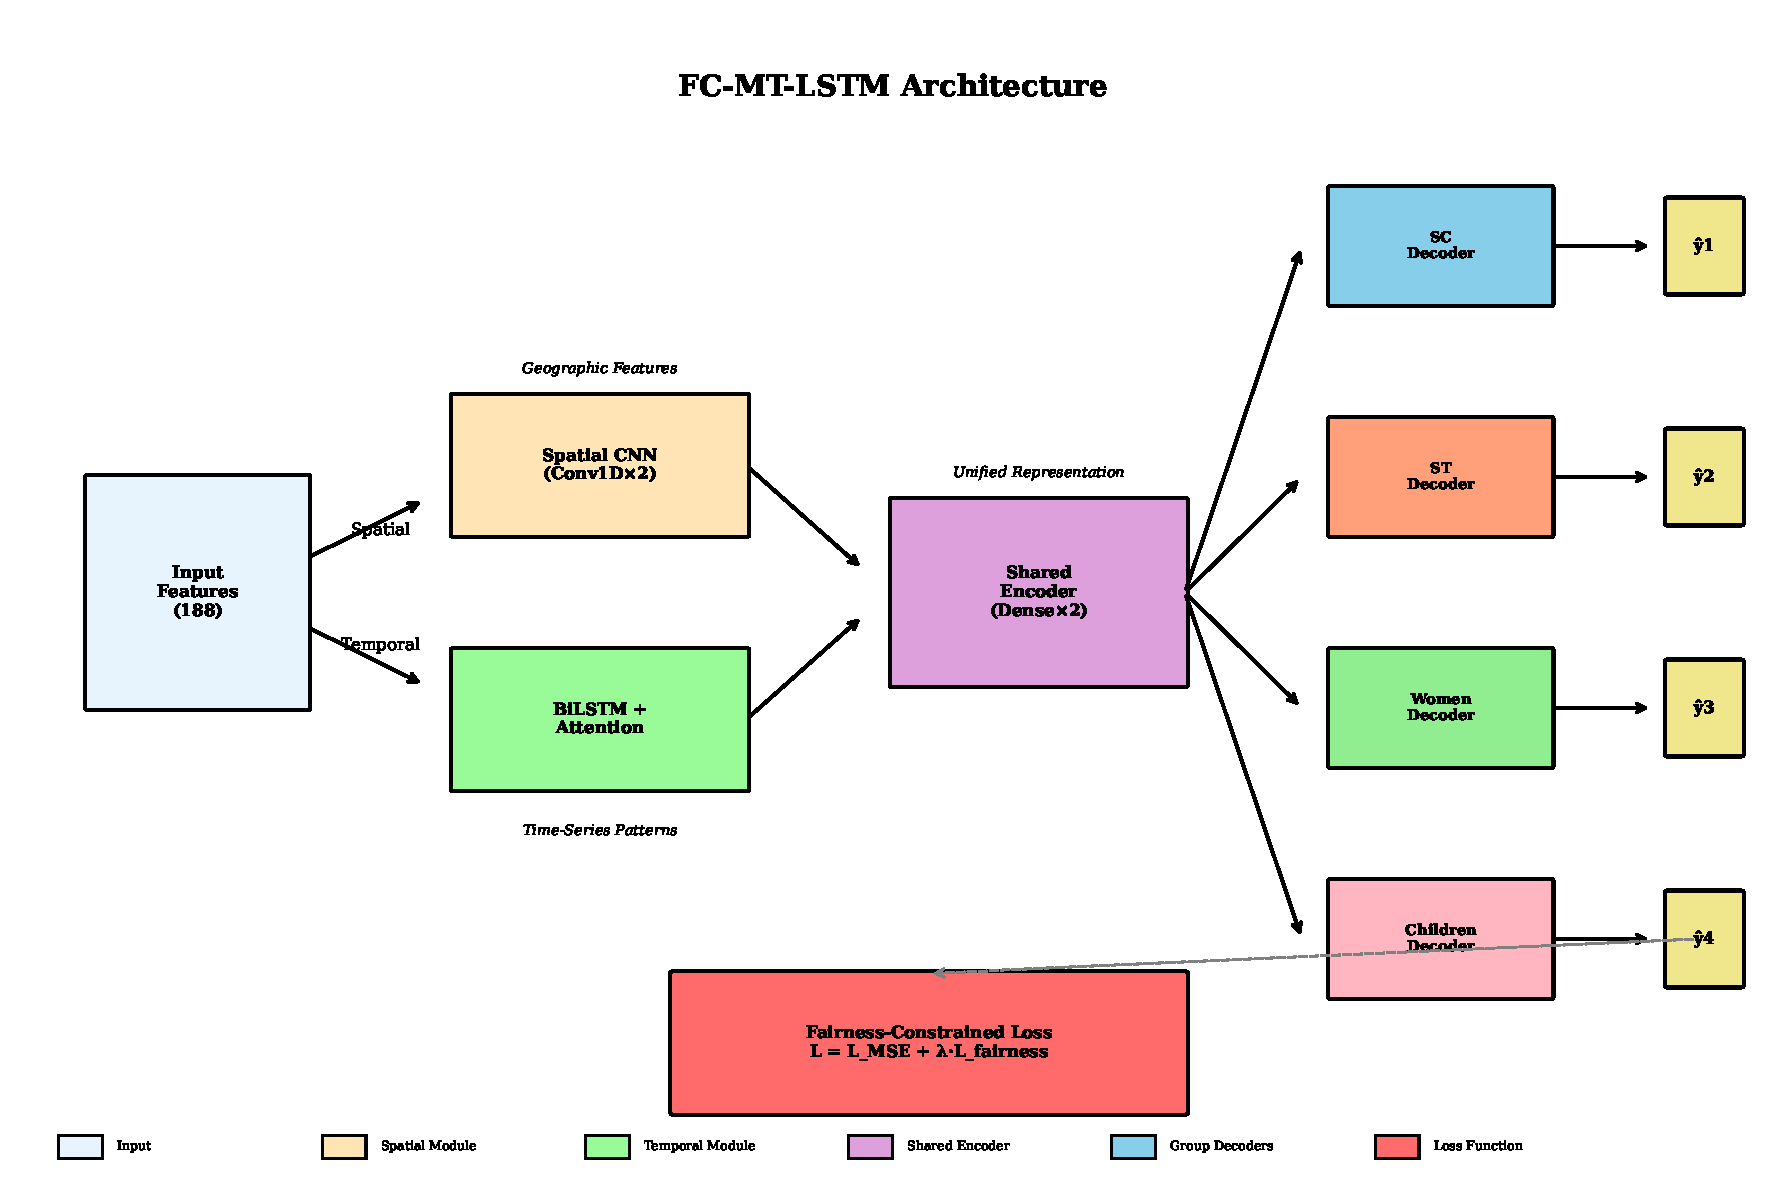
\includegraphics[width=\columnwidth]{figures/fig8_architecture.pdf}
\caption{FC-MT-LSTM Architecture. A CNN extracts spatial features and a bidirectional attention-based LSTM learns time-dependent patterns. Outputs are combined through a shared encoder and passed to four dedicated decoders. The objective incorporates fairness constraints so that both accuracy and group equity are jointly optimised.}
\label{fig:architecture}
\end{figure}

\subsection{Spatial CNN and Temporal Module}

The spatial CNN transforms $X_{\text{spatial}}$ via two 1D convolutions with batch normalisation and ReLU, followed by global max pooling and a dense layer to produce a compact spatial representation. The temporal module employs a bidirectional LSTM over $X_{\text{temporal}}$ with an additive attention mechanism that assigns weights $\alpha_t$ to each time step and produces a weighted sum $H_{\text{temporal}}$. The attention weights quantify each year's relevance to predicting future crime.

\subsection{Shared Encoder and Decoders}

The shared encoder concatenates $H_{\text{spatial}}$ and $H_{\text{temporal}}$ and passes them through two dense layers with batch normalisation, ReLU, and dropout, yielding a 256-dimensional representation. Four group-specific decoders, each with two dense layers and dropout, map this shared representation to predictions $\hat{y}_g$ for $g \in \{\text{SC, ST, Women, Children}\}$.

\subsection{Fairness-Constrained Loss and Training}

A balance between predictive fidelity and cross group parity:
\[
\mathcal{L}_{\text{total}} = \mathcal{L}_{\text{MSE}} + \lambda \mathcal{L}_{\text{fairness}},
\]
where $\lambda = 0.5$. The MSE term is
\[
\mathcal{L}_{\text{MSE}} = \frac{1}{B} \sum_{i=1}^{B} (y_i - \hat{y}_{g_i})^2,
\]
with $g_i$ denoting the protected group label. The fairness term penalises disparities in group-wise MAE:
\[
\mathcal{L}_{\text{fairness}} = \frac{1}{N_{\text{pairs}}} \sum_{g_1 < g_2} |\text{MAE}_{g_1} - \text{MAE}_{g_2}|,
\]
where $\text{MAE}_g$ is the mean absolute error for group $g$. This discourages regimes in which one protected group consistently experiences much larger errors than others.

We train \modelname{} with Adam (learning rate $0.001$, weight decay $10^{-5}$), batch size 32, up to 100 epochs with early stopping (patience 10), a StepLR schedule (factor 0.5 every 20 epochs), gradient clipping (max norm 1.0), and a 20\% validation split.

% ------------------------------------------------------------------
\section{Experimental Setup}
% ------------------------------------------------------------------

\subsection{Baseline Models}

We benchmark \modelname{} against:

\textbf{SARIMA}: Seasonal ARIMA(1,1,1)(1,1,1,12) models fitted per district–group.

\textbf{Prophet}: Changepoint prior scale 0.05 and a decomposition model with yearly seasonality \cite{taylor2018forecasting}.

\textbf{Random Forest}: 100 trees, maximum depth 10, minimum samples split 5 \cite{breiman2001random}.

\textbf{XGBoost}: 200 trees, maximum depth 6, learning rate 0.1 \cite{chen2016xgboost}.

\textbf{CNN-LSTM}: A 1D CNN of 32 filters which is followed by a two-layer LSTM with 64 hidden units.

\textbf{Transformer}: A sequence model with 2 encoder layers, 4 attention heads, and model dimension 64 \cite{vaswani2017attention}.

\subsection{Evaluation Metrics}

Model Accuracies are measured by Mean Absolute Error (MAE), Root Mean Square Error (RMSE), and coefficient of determination (R$^2$). Assesment is done through  Fairness Gap (difference between maximum and minimum group-wise MAE) and Fairness Ratio (quotient of maximum to minimum group-wise MAE). Lower Fairness Gap and Fairness Ratio (closer to 1.0) indicates more equitable performance across said groups.

% ------------------------------------------------------------------
\section{Results}
% ------------------------------------------------------------------

\subsection{Overall Performance}

Table~\ref{tab:overall_results} is a summary of test performance across models.

\begin{table*}[htbp]
\caption{Overall Model Performance Comparison on Test Set (2022)}
\label{tab:overall_results}
\centering
\begin{tabular}{lcccccc}
\toprule
\textbf{Model} & \textbf{MAE $\downarrow$} & \textbf{RMSE $\downarrow$} & \textbf{R$^2$ $\uparrow$} & \textbf{F. Gap $\downarrow$} & \textbf{F. Ratio $\downarrow$} & \textbf{Time (min)} \\
\midrule
SARIMA & 166.61 & 220.34 & 0.000 & 20.85 & 1.17 & 0.07 \\
Prophet & 135.46 & 198.19 & 0.191 & 17.60 & 1.22 & 1.41 \\
Random Forest & 2.14 & 5.63 & 0.9993 & 1.08 & 4.74 & 0.12 \\
XGBoost & \textbf{1.83} & \textbf{4.13} & \textbf{0.9996} & 0.81 & 3.73 & 0.12 \\
CNN-LSTM & 23.83 & 57.33 & 0.9419 & 0.00* & 1.00* & 4.16 \\
Transformer & 4.65 & 9.12 & 0.9985 & 0.00* & 1.00* & 6.90 \\
\midrule
\textbf{\modelname{} (Ours)} & 6.54 & 16.05 & 0.9922 & 12.61 & \textbf{1.99} & 8.50 \\
\bottomrule
\multicolumn{7}{l}{\footnotesize *CNN-LSTM and Transformer did not produce per-group breakdowns; 0.00/1.00 indicates missing evaluation.} \\
\multicolumn{7}{l}{\footnotesize Bold indicates best performance. $\downarrow$ = lower is better, $\uparrow$ = higher is better.}
\end{tabular}
\end{table*}

Leveraging mixed modelling methods (Random Forest, XGBoost) achieve the lowest aggregate errors (MAE below 2.5, R$^2$ above 0.999) but suffer fairness ratios between 3.73 and 4.74, meaning some protected groups are modelled worse than others. Classical time-series baseline models (SARIMA, Prophet) also perform poorly in both MAE and R$^2$ and offer only conceited fairness. \modelname{} relaxes aggregate accuracy (MAE 6.54, R$^2$ 0.9922) but nearly halves the fairness ratio relative to mix ones, yielding a more even distribution of errors across protected groups, comliant with the trade-off shown in Fig.~\ref{fig:tradeoff}.

\subsection{Per-Group Performance}

Table~\ref{tab:group_performance} presents the per-group breakdown for \modelname{}.

\begin{table}[htbp]
\caption{\modelname{} Per-Group Performance}
\label{tab:group_performance}
\centering
\begin{tabular}{lcccc}
\toprule
\textbf{Group} & \textbf{MAE} & \textbf{RMSE} & \textbf{R$^2$} & \textbf{Samples} \\
\midrule
SC & 2.08 & 3.15 & 0.9673 & 16 \\
ST & 1.40 & 1.54 & 0.0000 & 15 \\
Women & 7.89 & 10.81 & 0.9981 & 16 \\
Children & 14.01 & 29.12 & 0.9852 & 17 \\
\midrule
\textbf{Overall} & \textbf{6.54} & \textbf{16.05} & \textbf{0.9922} & \textbf{64} \\
\bottomrule
\end{tabular}
\end{table}

Group-specific MAE ranges from 1.40 (ST) to 14.01 (children). The higher error for children reflects the difficulty of predicting crimes against minors, which span more categories than for other groups. Within more comparable groups (SC, ST, women), disparities remain substantially smaller than those observed for ensemble baselines.

\begin{figure}[htbp]
\centering
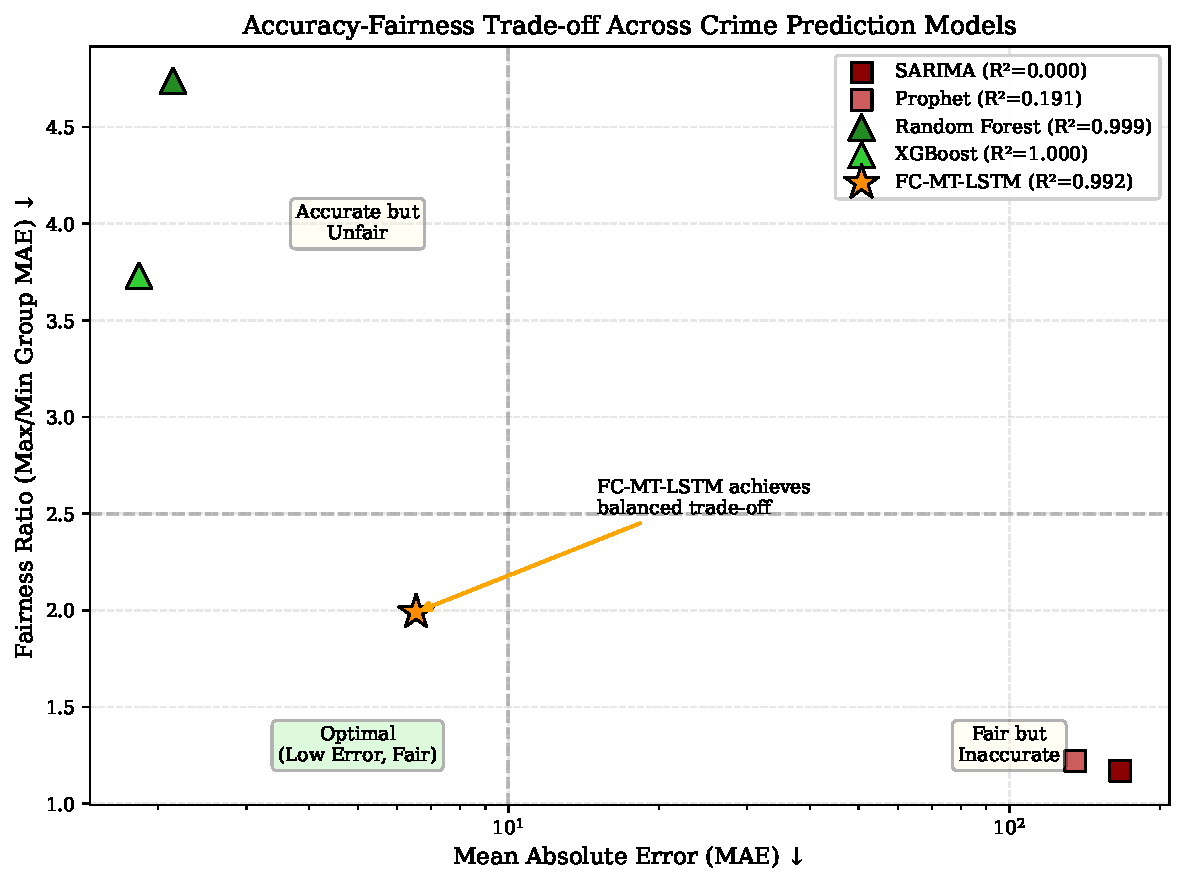
\includegraphics[width=\columnwidth]{figures/fig2_accuracy_fairness_tradeoff.pdf}
\caption{Accuracy–Fairness Trade-off. Models are positioned by MAE (x-axis, log scale) and Fairness Ratio (y-axis). The ideal region (low error, low unfairness) lies at the bottom-left. \modelname{} offers a balanced compromise between aggregate accuracy and group-level equity.}
\label{fig:tradeoff}
\end{figure}

\subsection{Fairness–Accuracy Trade-off and Feature Importance}

Table~\ref{tab:features} reports the top predictive features for the ensemble baselines.

\begin{table}[htbp]
\caption{Top 5 Feature Importance}
\label{tab:features}
\centering
\begin{tabular}{lcc}
\toprule
\textbf{Feature} & \textbf{RF} & \textbf{XGBoost} \\
\midrule
Rolling Mean (3Y) & 0.591 & 0.759 \\
Rolling Mean (2Y) & 0.310 & 0.164 \\
YoY Change & 0.062 & 0.037 \\
Group Proportion & 0.031 & 0.025 \\
Rolling Std (2Y) & 0.004 & 0.009 \\
\bottomrule
\end{tabular}
\end{table}

The importance of historical trend features in each of the ensembles is substantial, and the contribution of the average variables in a rolling basis and the difference year over year is over 90\% of the total weight. Such strong dependence on previous patterns reveals why such models can simply continue repeating the same spatial and group biases unless we introduce justice in its training objectives.

% ------------------------------------------------------------------
\section{Discussion and Conclusion}
% ------------------------------------------------------------------
\subsection{Practical Implications}

I believe that the framework of \modelname{} is quite helpful with regards to policing and policy. It produces predictions in which errors remain more balanced within the groups under the protection and prevents over-policing of certain areas and ignoring other areas. The group-specific decoders enable practitioners to identify group-specific trends such as the ones that are specific to women or children so they can design group-relevant prevention programs rather than general ones.
Temporal attention layer also increases interpretability and defines the particular time spans which produce the most influential effect on predictive results.

\subsection{Limitations}

Biases from spotty reporting, uneven surveillance, and changing laws is carried in historical crime data; fairness training helps but won't eradicate them. Focusing on just four groups leaves joins--like caste, gender, and age--only incompletely addressed, with subgroup samples too less for fine detail. The model fits India's context, to use anywhere else will require retooling and testing.

\subsection{Ethics and Future Work}

These are dominated by ethical factors and high scores of fairness are not enough to sanction unregulated predictive systems (especially when communities Agencies have no agency over their use). Algorithms can be used to obscure prejudice because human actors are still responsible of any harm. The \modelname{} system is a decision-support system, a clear open-ended monitoring by the community is still required for any useful use.

The current paper presents a fairness-conscious multi-task LSTM architecture, namely, called \modelname{}, that allows crime prediction among four guarded groups. It combines spatial convolutional neural networks, layers with temporal attention, a common encoder and decoders that are specific to particular groups controlled by a fairness-penalised loss. Using NCRB data 20172022, the model performs better in cross-group error differences between accuracy-only ensemble baselines while maintaining aggregate performance.

Further research will be inclusive of causal fairness methods to differentiate noise and true  crimes, rebalance fairness weights based on demographic changes, and multi-task learning to understand overlapping group processes. Calibration would also be further improved by incorporation of Bayesian uncertainty estimates.

Finally, the implementation of the tools like \modelname{} implies institutional changes, extensive legal examination, and effective involvement of the community to the extent that can truly promote the cause of fair justice.

% ------------------------------------------------------------------
\section*{Acknowledgment}
% ------------------------------------------------------------------

The authors thank the National Crime Records Bureau (NCRB) of India for making crime statistics publicly available.

% ------------------------------------------------------------------
\section*{Declarations}
% ------------------------------------------------------------------

\begin{itemize}
\item \textbf{Funding}: This research received no specific grant from any funding agency in the public, commercial, or not-for-profit sectors.
\item \textbf{Conflicts of Interest}: The authors declare that they have no known competing financial interests or personal relationships that could have appeared to influence the work reported in this paper.
\item \textbf{Ethics Approval}: Not applicable. This study uses publicly available aggregated crime statistics from the NCRB and does not involve human participants, animal experiments, or sensitive personal data.
\item \textbf{Consent to Participate and Consent for Publication}: Not applicable.
\item \textbf{Availability of Data and Material}: The datasets analysed in this study are publicly available from the National Crime Records Bureau (NCRB) website: \url{https://ncrb.gov.in/}.
\item \textbf{Code Availability}: The source code for the \modelname{} model is implemented in PyTorch and TensorFlow and is available upon reasonable request from the corresponding author.
\end{itemize}

% ------------------------------------------------------------------
\begin{thebibliography}{26}
% ------------------------------------------------------------------

\bibitem{perry2013predictive}
W.~L. Perry, B.~McInnis, C.~C. Price, S.~C. Smith, and J.~S. Hollywood, ``Predictive policing: The role of crime forecasting in law enforcement operations,'' RAND Corporation, 2013.

\bibitem{lum2016predict}
K.~Lum and W.~Isaac, ``To predict and serve?'' \textit{Significance}, vol.~13, no.~5, pp.~14--19, 2016.

\bibitem{richardson2019dirty}
R.~Richardson, J.~M. Schultz, and K.~Crawford, ``Dirty data, bad predictions: How civil rights violations impact police data, predictive policing systems, and justice,'' \textit{New York University Law Review Online}, vol.~94, pp.~192--233, 2019.

\bibitem{wu2024improving}
J.~Wu and V.~Frias-Martinez, ``Improving the fairness of deep-learning, short-term crime prediction with under-reporting-aware models,'' \textit{arXiv preprint arXiv:2406.04382}, 2024.

\bibitem{angwin2016machine}
J.~Angwin, J.~Larson, S.~Mattu, and L.~Kirchner, ``Machine bias,'' \textit{ProPublica}, May 2016.

\bibitem{barocas2016big}
S.~Barocas and A.~D. Selbst, ``Big data's disparate impact,'' \textit{California Law Review}, vol.~104, no.~3, pp.~671--732, 2016.

\bibitem{box2015time}
G.~E. Box, G.~M. Jenkins, G.~C. Reinsel, and G.~M. Ljung, \textit{Time Series Analysis: Forecasting and Control}, 5th~ed. John Wiley \& Sons, 2015.

\bibitem{anselin2000spatial}
L.~Anselin, J.~Cohen, D.~Cook, W.~Gorr, and G.~Tita, ``Spatial analyses of crime,'' \textit{Criminal Justice}, vol.~4, no.~2, pp.~213--262, 2000.

\bibitem{breiman2001random}
L.~Breiman, ``Random forests,'' \textit{Machine Learning}, vol.~45, no.~1, pp.~5--32, 2001.

\bibitem{taylor2018forecasting}
S.~J. Taylor and B.~Letham, ``Forecasting at scale,'' \textit{The American Statistician}, vol.~72, no.~1, pp.~37--45, 2018.

\bibitem{huang2018deepcrime}
C.~Huang, J.~Zhang, Y.~Zheng, and N.~V. Chawla, ``DeepCrime: Attentive hierarchical recurrent networks for crime prediction,'' in \textit{Proc. ACM CIKM}, 2018, pp.~1423--1432.

\bibitem{hochreiter1997long}
S.~Hochreiter and J.~Schmidhuber, ``Long short-term memory,'' \textit{Neural Computation}, vol.~9, no.~8, pp.~1735--1780, 1997.

\bibitem{vaswani2017attention}
A.~Vaswani \etal, ``Attention is all you need,'' in \textit{Advances in Neural Information Processing Systems}, vol.~30, 2017, pp.~5998--6008.

\bibitem{dressel2018accuracy}
J.~Dressel and H.~Farid, ``The accuracy, fairness, and limits of predicting recidivism,'' \textit{Science Advances}, vol.~4, no.~1, p.~eaao5580, 2018.

\bibitem{verma2018fairness}
S.~Verma and J.~Rubin, ``Fairness definitions explained,'' in \textit{Proc. Int. Workshop on Software Fairness}, 2018, pp.~1--7.

\bibitem{kleinberg2016inherent}
J.~Kleinberg, S.~Mullainathan, and M.~Raghavan, ``Inherent trade-offs in the fair determination of risk scores,'' \textit{arXiv preprint arXiv:1609.05807}, 2016.

\bibitem{kamiran2012data}
F.~Kamiran and T.~Calders, ``Data preprocessing techniques for discrimination prevention,'' \textit{Knowledge and Information Systems}, vol.~33, no.~1, pp.~1--33, 2012.

\bibitem{zafar2017fairness}
M.~B. Zafar, I.~Valera, M.~Gomez~Rodriguez, and K.~P. Gummadi, ``Fairness constraints: Mechanisms for fair classification,'' in \textit{Proc. AISTATS}, 2017, pp.~962--970.

\bibitem{hardt2016equality}
M.~Hardt, E.~Price, and N.~Srebro, ``Equality of opportunity in supervised learning,'' in \textit{Advances in Neural Information Processing Systems}, vol.~29, 2016, pp.~3315--3323.

\bibitem{caruana1997multitask}
R.~Caruana, ``Multitask learning,'' \textit{Machine Learning}, vol.~28, no.~1, pp.~41--75, 1997.

\bibitem{zhang2021survey}
Y.~Zhang and Q.~Yang, ``A survey on multi-task learning,'' \textit{IEEE Trans. Knowledge and Data Engineering}, vol.~34, no.~12, pp.~5586--5609, 2021.

\bibitem{chen2016xgboost}
T.~Chen and C.~Guestrin, ``XGBoost: A scalable tree boosting system,'' in \textit{Proc. 22nd ACM SIGKDD Int. Conf. on Knowledge Discovery and Data Mining (KDD '16)}, 2016, pp.~785--794.

\end{thebibliography}

\end{document}

